\documentclass{beamer}
\usetheme{Madrid}
\usepackage{amsmath, amssymb, tikz, bm, amsfonts, multicol}
\usepackage{graphicx, xcolor}
\usepackage{tikz}
\setcounter{MaxMatrixCols}{20}

\title[FYP]{Coherent Closure on Non-Distance Regular Graphs}
\author{Ho Jing Rui}
\institute[NTU]{Nanyang Technological University}
\date{April 22, 2025}

\begin{document}

\begin{frame}
  \titlepage
\end{frame}

%---------------------------------------------------------
\begin{frame}{Historical Motivation}
\begin{columns}

  % Left column: text
  \begin{column}{0.6\textwidth}
    \textbf{Euler's 36 Officers Problem (1782):}
    \begin{itemize}
      \item Arrange 36 officers in a \(6 \times 6\) square.
      \item 6 ranks × 6 regiments.
      \item Each row and column must contain \textit{exactly} one of each rank and regiment.
      \item Euler conjectured this is impossible (now proven true).
    \end{itemize}

    \vspace{1em}
    \textit{This inspired the study of MOLS,}
    
    \textit{Mutually Orthogonal Latin Squares.}
  \end{column}

  % Right column: image
  \begin{column}{0.4\textwidth}
    \centering
    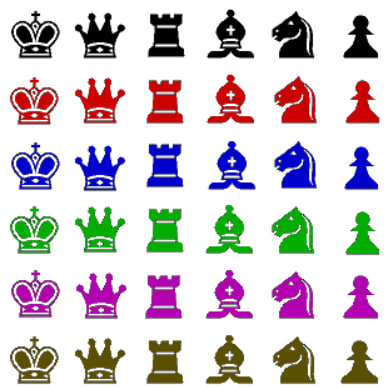
\includegraphics[width=\textwidth]{slides/bigsix.jpg}
  \end{column}

\end{columns}
\end{frame}

%---------------------------------------------------------
\begin{frame}{What Are MOLS?}
  \begin{itemize}
    \item A \textbf{Latin square}, $L$ of order \(n\) is a \(n \times n\) grid filled with \(n\) symbols, with no repeats per row or column.
    \item Two Latin squares, $L^{(1)}$ and $L^{(2)}$ are \textbf{orthogonal} if pairs \((L^{(1)}_{i,j}, L^{(2)}_{i,j})\) are all distinct.
    \item A set of Latin squares is \textbf{mutually orthogonal} if every pair of Latin squares in the set are orthogonal to each other.
  \end{itemize}
\end{frame}


%---------------------------------------------------------
\begin{frame}{MOLS(4)}
\[
\begin{aligned}
    L^{(1)} = \begin{bmatrix}
        1 & 2 & 3 & 4\\
        2 & 1 & 4 & 3\\
        3 & 4 & 1 & 2\\
        4 & 3 & 2 & 1
    \end{bmatrix},\quad 
    L^{(2)} = \begin{bmatrix}
        1 & 2 & 3 & 4\\
        4 & 3 & 2 & 1\\
        2 & 1 & 4 & 3\\
        3 & 4 & 1 & 2
    \end{bmatrix},\quad
    L^{(3)} = \begin{bmatrix}
        1&2&3&4\\
        3&4&1&2\\
        4&3&2&1\\
        2&1&4&3
    \end{bmatrix};
\end{aligned}
\]

\[
\begin{aligned}
    L^{\{1,2\}} =
    \begin{bmatrix}
        (1,1) & (2,2) & (3,3) & (4,4)\\
        (2,4) & (1,3) & (4,2) & (3,1)\\
        (3,2) & (4,1) & (1,4) & (2,3)\\
        (4,3) & (3,4) & (2,1) & (1,2)
    \end{bmatrix}.
\end{aligned}
\]
\end{frame}

%---------------------------------------------------------
\begin{frame}{MOLS(4)}
\[
\begin{aligned}
    L^{(1)} = \begin{bmatrix}
        1 & 2 & 3 & 4\\
        2 & 1 & 4 & 3\\
        3 & 4 & 1 & 2\\
        4 & 3 & 2 & 1
    \end{bmatrix},\quad 
    L^{(2)} = \begin{bmatrix}
        1 & 2 & 3 & 4\\
        4 & 3 & 2 & 1\\
        2 & 1 & 4 & 3\\
        3 & 4 & 1 & 2
    \end{bmatrix},\quad
    L^{(3)} = \begin{bmatrix}
        1&2&3&4\\
        3&4&1&2\\
        4&3&2&1\\
        2&1&4&3
    \end{bmatrix};
\end{aligned}
\]

\[
\begin{aligned}
    L^{\{1,3\}} =
    \begin{bmatrix}
        (1,1) & (2,2) & (3,3) & (4,4)\\
        (2,3) & (1,4) & (4,1) & (3,2)\\
        (3,4) & (4,3) & (1,2) & (2,1)\\
        (4,2) & (3,1) & (2,4) & (1,3)
    \end{bmatrix}.
\end{aligned}
\]
\end{frame}

%---------------------------------------------------------
\begin{frame}{MOLS(4)}
\[
\begin{aligned}
    L^{(1)} = \begin{bmatrix}
        1 & 2 & 3 & 4\\
        2 & 1 & 4 & 3\\
        3 & 4 & 1 & 2\\
        4 & 3 & 2 & 1
    \end{bmatrix},\quad 
    L^{(2)} = \begin{bmatrix}
        1 & 2 & 3 & 4\\
        4 & 3 & 2 & 1\\
        2 & 1 & 4 & 3\\
        3 & 4 & 1 & 2
    \end{bmatrix},\quad
    L^{(3)} = \begin{bmatrix}
        1&2&3&4\\
        3&4&1&2\\
        4&3&2&1\\
        2&1&4&3
    \end{bmatrix};
\end{aligned}
\]

\[
\begin{aligned}
    L^{\{2,3\}} =
    \begin{bmatrix}
        (1,1) & (2,2) & (3,3) & (4,4)\\
        (4,3) & (3,4) & (2,1) & (1,2)\\
        (2,4) & (1,3) & (4,2) & (3,1)\\
        (3,2) & (4,1) & (1,4) & (2,3)
    \end{bmatrix}.
\end{aligned}
\]
\end{frame}

% %---------------------------------------------------------
% \begin{frame}{MOLS and Orthogonal Arrays}
%   \begin{itemize}
%     \item Given a set of \(m-2\) MOLS($n$), we can write the rows, columns and symbols of each $L^{(i)}_{r,c},i\in[m-2]$ by the following tuple:
%     \[
%     \begin{pmatrix}
%         r&c&L^{(1)}_{r,c}&L^{(2)}_{r,c}&\cdots&L^{(m-2)}_{r,c}
%     \end{pmatrix}
%     \]
%     \item Taking the transpose, we note that this is a column in an orthogonal array with parameters $(m,n)$.
%   \end{itemize}
% \end{frame}


%---------------------------------------------------------
\begin{frame}{What is an Orthogonal Array?}
  \textbf{Definition:} An \textbf{orthogonal array} \( \text{OA}(m, n) \) is an \( m \times n^2 \) array over \( [n] \), such that:
  \begin{itemize}
    \item Every pair of rows contains each tuple of $[n]\times[n]$ exactly once.
  \end{itemize}

  \vspace{1em}
  We can build OA$(m,n)$ by using a set of $m-2$ MOLS($n$), $\left\{L^{(1)},\dots, L^{(m-2)}\right\}$, and write their symbols in such a manner:
  \begin{equation*}
      \operatorname{OA}(m,n) = \begin{bmatrix}
          1&1&\dots&r&\dots&n&n\\
          1&2&\dots&c&\dots&n-1&n\\
          L_{1,1}^{(1)}&L_{1,2}^{(1)}&\dots&L_{r,c}^{(1)}&\dots&L_{n,n-1}^{(1)}&L_{n,n}^{(1)}\\
          \vdots&\vdots&\vdots&\vdots&\vdots&\vdots&\vdots\\
          L_{1,1}^{(m-2)}&L_{1,2}^{(m-2)}&\dots&L_{r,c}^{(m-2)}&\dots&L_{n,n-1}^{(m-2)}&L_{n,n}^{(m-2)}
      \end{bmatrix}.
  \end{equation*}
\end{frame}

%------------------------------------------------------------
\begin{frame}{Block Graph}
  \textbf{Definition:} A \textbf{block graph} induced by an orthogonal array $\text{OA}(m,n)$ is a simple graph $G=(V,E)$ with the following properties:
  \begin{itemize}
      \item $|V| = n^2$;
      \item Vertices are labeled by tuples $(r, c)$ where $r, c \in [n]$;
      \item Two vertices $(r_1, c_1)$ and $(r_2, c_2)$ are adjacent, i.e., $(r_1, c_1) \sim (r_2, c_2)$, if and only if:
      \vspace{0.5em}
      \begin{center}
        the tuples 
        $\displaystyle \left(r_1, c_1, L^{(1)}_{r_1, c_1}, \dots, L^{(m-2)}_{r_1, c_1} \right)$ and 
        $\displaystyle \left(r_2, c_2, L^{(1)}_{r_2, c_2}, \dots, L^{(m-2)}_{r_2, c_2} \right)$
        agree in exactly one coordinate.
      \end{center}
  \end{itemize}
\end{frame}


%---------------------------------------------------------
\begin{frame}{Example of OA(3,3)}
  \begin{itemize}
    \item Consider this Latin Square of order 3:
    \[
    \begin{aligned}
        L = \begin{bmatrix}
            1&2&3\\
            3&1&2\\
            2&3&1
        \end{bmatrix}.
    \end{aligned}
    \]
    \item Construct OA(3,3) with each column: 
    $\begin{bmatrix}
    \textcolor{red}{\text{row}}\\
    \textcolor{blue}{\text{column}}\\
    L_{\text{row},\text{column}}\end{bmatrix}$
    \[
    \begin{aligned}
        \text{OA}(3,3) = \begin{bmatrix}
            \textcolor{red}{1}&\textcolor{red}{1}&\textcolor{red}{1}&\textcolor{red}{2}&\textcolor{red}{2}&\textcolor{red}{2}&\textcolor{red}{3}&\textcolor{red}{3}&\textcolor{red}{3}\\
            \textcolor{blue}{1}&\textcolor{blue}{2}&\textcolor{blue}{3}&\textcolor{blue}{1}&\textcolor{blue}{2}&\textcolor{blue}{3}&\textcolor{blue}{1}&\textcolor{blue}{2}&\textcolor{blue}{3}\\
            1&2&3&3&1&2&2&3&1
        \end{bmatrix}.
    \end{aligned}
    \]
  \end{itemize}
\end{frame}

%---------------------------------------------------------
% \begin{frame}{Example of OA(3,3)}
% \[
% \begin{aligned}
%     \text{OA}(3,3) = \begin{bmatrix}
%         \textcolor{red}{1}&\textcolor{red}{1}&\textcolor{red}{1}&\textcolor{red}{2}&\textcolor{red}{2}&\textcolor{red}{2}&\textcolor{red}{3}&\textcolor{red}{3}&\textcolor{red}{3}\\
%         \textcolor{blue}{1}&\textcolor{blue}{2}&\textcolor{blue}{3}&\textcolor{blue}{1}&\textcolor{blue}{2}&\textcolor{blue}{3}&\textcolor{blue}{1}&\textcolor{blue}{2}&\textcolor{blue}{3}\\
%         1&2&3&3&1&2&2&3&1
%     \end{bmatrix}
% \end{aligned}
% \]
% \begin{itemize}
%     \item We treat each column as a vertex, and 2 columns $v_1=\begin{bmatrix}
%         r_1\\c_1\\L_{r_1,c_1}
%     \end{bmatrix}$ and $v_2=\begin{bmatrix}
%         r_2\\c_2\\L_{r_2,c_2}
%     \end{bmatrix}$ are adjacent under the following rules:
%     \begin{equation*}
%         v_1\sim v_2 \iff 
%         \begin{bmatrix}
%         r_1\\c_1\\L_{r_1,c_1}
%     \end{bmatrix}\text{ and } \begin{bmatrix}
%         r_2\\c_2\\L_{r_2,c_2}
%     \end{bmatrix} \text{ agree in exactly one position}
%     \end{equation*}
% \end{itemize}
    
% \end{frame}
%---------------------------------------------------------
\begin{frame}{Example of OA(3,3)}
\centering
OA$(3,3)$ and its block graph

\vspace{1em}

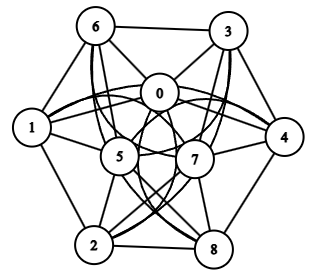
\includegraphics[width=0.4\textwidth]{slides/graph.png}

\[
\begin{aligned}
    \text{OA}(3,3) = \begin{bmatrix}
        \textcolor{red}{1}&\textcolor{red}{1}&\textcolor{red}{1}&\textcolor{red}{2}&\textcolor{red}{2}&\textcolor{red}{2}&\textcolor{red}{3}&\textcolor{red}{3}&\textcolor{red}{3}\\
        \textcolor{blue}{1}&\textcolor{blue}{2}&\textcolor{blue}{3}&\textcolor{blue}{1}&\textcolor{blue}{2}&\textcolor{blue}{3}&\textcolor{blue}{1}&\textcolor{blue}{2}&\textcolor{blue}{3}\\
        1&2&3&3&1&2&2&3&1
    \end{bmatrix}.
\end{aligned}
\]
\end{frame}



%---------------------------------------------------------
\begin{frame}{Base Case: Block Graph of OA(2,3)}

\vspace{1em}
\textit{This smaller case of a block graph guides our construction of more complex graphs.}

\vspace{1em}

\begin{columns}
  \begin{column}{0.6\textwidth}
    \begin{align*}
    &\text{OA}(2,3) \\=
    &\begin{bmatrix}
    1 & 1 & 1 & 2 & 2 & 2 & 3 & 3 & 3 \\
    1 & 2 & 3 & 1 & 2 & 3 & 1 & 2 & 3 
    \end{bmatrix}
    \end{align*}
  \end{column}

  \begin{column}{0.4\textwidth}
    \centering
    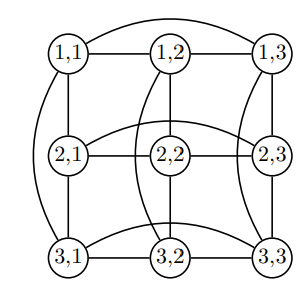
\includegraphics[width=\textwidth]{slides/r3.png}
  \end{column}
\end{columns}
\end{frame}



%---------------------------------------------------------
\begin{frame}{Rook Graphs: Definition}

    \textbf{Definition:} The \textbf{rook graph} \( R(n) \) is the block graph induced by OA$(2,n)$, $n\geq2$. 
  \begin{itemize}
    \item Vertices represent an $n\times n$ chessboard;
    \item Edges can be interpreted as possible moves for a rook to move on the chessboard.
  \end{itemize}

    \vspace{1em}
  \begin{columns}
      \begin{column}{0.7\textwidth}
            \[
            \begin{aligned}
                A(R(n)) = \underbrace{
                \left[
                    \begin{array}{cccc}
                    J_{n} - I & I_n & \cdots & I_n \\
                    I_n & J_n - I & \cdots & I_n \\
                    \vdots & \vdots & \ddots & \vdots \\
                    I_n & I_n & \cdots & J_n - I
                    \end{array}
                \right].
                }_{\text{\( n \) blocks}}
            \end{aligned}
            \]
      \end{column}

      \begin{column}{0.3\textwidth}
        \centering

        $R(8)$
        
        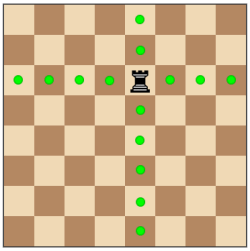
\includegraphics[width=0.8\textwidth]{slides/rook-moves.png}
    \end{column}
  \end{columns}
\end{frame}

%--------------------------------------------------------
\begin{frame}{Coherent Configurations}
    Let $V$ be a finite set and $\mathcal{R}=\{R_1,\dots,R_r\}$ be a set of binary relations. For each $R_i$, let $W_i\in\operatorname{Mat}_V(\{0,1\})$ be defined such that its 
    
    $(x,y)$ entry is 1 if $(x,y)\in R_i$ and 0 otherwise. Suppose the following 4 conditions

    \vspace{0.8em}
    \begin{itemize}
        \item \( \sum_{i=1}^{r} W_i = J \);
        \item For each \( i \in [r] \), there exists \( j \in [r] \) such that \( W_i^T = W_j \);
        \item There exists a subset \( \Delta \subseteq [r] \) such that \( \sum_{i \in \Delta} W_i = I \);
        \item \( W_i W_j = \sum_{k=1}^{r} p^k_{i,j} W_k \) for some constants \( p^k_{i,j} \in \mathbb{Z}_{\geq 0} \), for all \( i, j \in [r] \).
    \end{itemize}
    
    \vspace{0.8em}
    Then $(V,\mathcal{R})$ is called a \textbf{coherent configuration} of \textbf{rank} $|\mathcal{R}|=r$.
\end{frame}

%---------------------------------------------------------
\begin{frame}{Coherent Algebras}
    \textbf{Definition:} A matrix algebra $\mathcal{A}\subset\operatorname{Mat}(\mathbb{C})$ satisfies the following:
  \begin{itemize}
    \item Spanned by unique basis $\{0,1\}$-matrices: \(\{ A_1, \dots, A_r \}\);
    \item Closed under matrix multiplication, transpose, and Hadamard product;
    \item $I,J\in\mathcal{A}$.
  \end{itemize}

  We say $\mathcal{A}(G)$ is a \textbf{coherent algebra} containing the adjacency matrix of $G$ when we talk about coherent algebras in this presentation.
\end{frame}

%----------------------------------------------------------
\begin{frame}{Coherent Algebras}
    \textbf{Key Property:} If \( \mathcal{A}_1 \), \( \mathcal{A}_2 \) are coherent algebras containing the adjacency matrix of a graph $G$,
    then \(\mathcal{A}' =  \mathcal{A}_1 \cap \mathcal{A}_2 \) is also a coherent algebra containing the adjacency matrix of a graph $G$.
    
    \vspace{1em}
    \textit{Thus, we are motivated to find the minimal coherent algebra, which we call the coherent closure}.
\end{frame}

%---------------------------------------------------------
\begin{frame}{Coherent Closure, \texorpdfstring{$\mathcal{W}(G)$}{W(G)}}
    \textbf{Definition:} The minimal coherent algebra containing the adjacency matrix of a graph $G=(V,E)$ is called the \textbf{coherent closure}, and denoted as $\mathcal{W}(G)$.
    
    \vspace{1em}
    \textbf{Properties:}
    \begin{itemize}
        \item $A(G)\in\mathcal{W}(G)$;
        \item Basis matrices, $\{W_1,W_2\dots,W_r\}$, represent structural relations in the graph;
        \item The number of basis matrices in the coherent closure is called the \textbf{coherent rank} of $G$. 
        \begin{equation*}
            \operatorname{cr}(G) = |\mathcal{W}(G)| = r.
        \end{equation*}
    \end{itemize}
    
    \vspace{0.8em}
    \textit{We investigate how this algebra changes under graph operations that disrupt the regularity of a graph.}
\end{frame}

%-------------------------------------------------------------
\begin{frame}{2-WL Refinement Algorithm}
    \begin{columns}
        \begin{column}{0.7\textwidth}
        \begin{align*}
            A_1 = \begin{bmatrix}
                a&b&c&b\\
                b&a&b&b\\
                c&b&a&b\\
                b&b&b&a
            \end{bmatrix}
        \end{align*}
        \end{column}

        \begin{column}{0.3\textwidth}
            \centering
            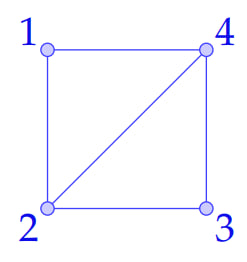
\includegraphics[width=0.7\textwidth]{slides/pic_1.jpg}
        \end{column}
    \end{columns}
    
    \vspace{1em}
    
\end{frame}
\addtocounter{framenumber}{-1}
%-------------------------------------------------------------
\begin{frame}{2-WL Refinement Algorithm}
    \begin{columns}
        \begin{column}{0.7\textwidth}
        \begin{align*}
            A_1 = \begin{bmatrix}
                a&b&c&b\\
                b&a&b&b\\
                c&b&a&b\\
                b&b&b&a
            \end{bmatrix}
        \end{align*}
        \end{column}

        \begin{column}{0.3\textwidth}
            \centering
            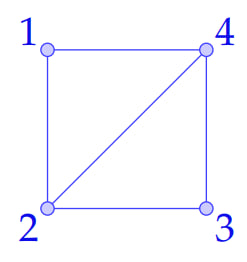
\includegraphics[width=0.7\textwidth]{slides/pic_1.jpg}
        \end{column}
    \end{columns}
    
    \vspace{1em}
    \[
    \scalebox{0.8}{
    $
        A_1^2 = \begin{bmatrix}
            a^2+2b^2+c^2 & ab+ba+b^2+cb&ac+2b^2+ca & ab+ba+b^2+cb\\
            ab+ba+b^2+bc&a^2+3b^2 & ab+ba+b^2+bc & ab+ba+2b^2\\
            ac+2b^2+ca&ab+ba+b^2+cb&a^2+2b^2+c^2&ab+ba+b^2+cb\\
            ab+ba+b^2+bc&ab+ba+2b^2&ab+ba+b^2+bc&a^2+3b^2
        \end{bmatrix}
    $
    }
    \]
    
\end{frame}
\addtocounter{framenumber}{-1}

%-------------------------------------------------------------
\begin{frame}{2-WL Refinement Algorithm}
    \begin{columns}
        \begin{column}{0.7\textwidth}
        \begin{align*}
            A_1 = \begin{bmatrix}
                a&b&c&b\\
                b&a&b&b\\
                c&b&a&b\\
                b&b&b&a
            \end{bmatrix}
        \end{align*}
        \end{column}

        \begin{column}{0.3\textwidth}
            \centering
            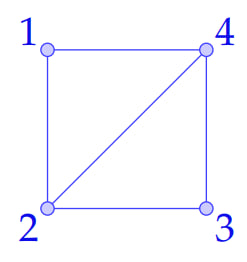
\includegraphics[width=0.7\textwidth]{slides/pic_1.jpg}
        \end{column}
    \end{columns}
    
    \vspace{1em}
    \[
    \scalebox{0.8}{
    $
        A_1^2 = \begin{bmatrix}
            \textcolor{red}{a^2+2b^2+c^2} &ab+ba+b^2+cb&ac+2b^2+ca & ab+ba+b^2+cb\\
            ab+ba+b^2+bc&a^2+3b^2 & ab+ba+b^2+bc & ab+ba+2b^2\\
            ac+2b^2+ca&ab+ba+b^2+cb&\textcolor{red}{a^2+2b^2+c^2}&ab+ba+b^2+cb\\
            ab+ba+b^2+bc&ab+ba+2b^2&ab+ba+b^2+bc&a^2+3b^2
        \end{bmatrix}
    $
    }
    \]

    \vspace{1em}
    \begin{align*}
        A_2 = \begin{bmatrix}
            \textcolor{red}{a}& & & \\
             & & & \\
             & &\textcolor{red}{a}& \\
             & & & \\
        \end{bmatrix}
    \end{align*}
\end{frame}
\addtocounter{framenumber}{-1}
%-------------------------------------------------------------
\begin{frame}{2-WL Refinement Algorithm}
    \begin{columns}
        \begin{column}{0.7\textwidth}
        \begin{align*}
            A_1 = \begin{bmatrix}
                a&b&c&b\\
                b&a&b&b\\
                c&b&a&b\\
                b&b&b&a
            \end{bmatrix}
        \end{align*}
        \end{column}

        \begin{column}{0.3\textwidth}
            \centering
            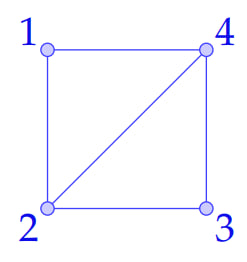
\includegraphics[width=0.7\textwidth]{slides/pic_1.jpg}
        \end{column}
    \end{columns}
    
    \vspace{1em}
    \[
    \scalebox{0.8}{
    $
        A_1^2 = \begin{bmatrix}
            {a^2+2b^2+c^2} & \textcolor{blue}{ab+ba+b^2+cb}&ac+2b^2+ca & \textcolor{blue}{ab+ba+b^2+cb}\\
            ab+ba+b^2+bc&a^2+3b^2 & ab+ba+b^2+bc & ab+ba+2b^2\\
            ac+2b^2+ca&\textcolor{blue}{ab+ba+b^2+cb}&a^2+2b^2+c^2&\textcolor{blue}{ab+ba+b^2+cb}\\
            ab+ba+b^2+bc&ab+ba+2b^2&ab+ba+b^2+bc&a^2+3b^2
        \end{bmatrix}
    $
    }
    \]

    \vspace{1em}
    \begin{align*}
        A_2 = \begin{bmatrix}
            a&\textcolor{blue}{b}& &\textcolor{blue}{b}\\
             && &\\
             &\textcolor{blue}{b} &a&\textcolor{blue}{b} \\
             & & & \\
        \end{bmatrix}
    \end{align*}
\end{frame}
\addtocounter{framenumber}{-1}
%-------------------------------------------------------------
\begin{frame}{2-WL Refinement Algorithm}
    \begin{columns}
        \begin{column}{0.7\textwidth}
        \begin{align*}
            A_1 = \begin{bmatrix}
                a&b&c&b\\
                b&a&b&b\\
                c&b&a&b\\
                b&b&b&a
            \end{bmatrix}
        \end{align*}
        \end{column}

        \begin{column}{0.3\textwidth}
            \centering
            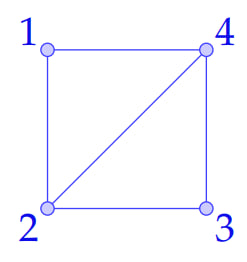
\includegraphics[width=0.7\textwidth]{slides/pic_1.jpg}
        \end{column}
    \end{columns}
    
    \vspace{1em}
    \[
    \scalebox{0.8}{
    $
        A_1^2 = \begin{bmatrix}
            a^2+2b^2+c^2 & ab+ba+b^2+cb&ac+2b^2+ca & ab+ba+b^2+cb\\
            ab+ba+b^2+bc&a^2+3b^2 & ab+ba+b^2+bc & ab+ba+2b^2\\
            ac+2b^2+ca&ab+ba+b^2+cb&a^2+2b^2+c^2&ab+ba+b^2+cb\\
            ab+ba+b^2+bc&ab+ba+2b^2&ab+ba+b^2+bc&a^2+3b^2
        \end{bmatrix}
    $
    }
    \]

    \vspace{1em}
    \begin{align*}
        A_2 = \begin{bmatrix}
            a&b&c&b\\
            d&e&d&f\\
            c&b&a&b\\
            d&f&d&e
        \end{bmatrix}
    \end{align*}
\end{frame}
\addtocounter{framenumber}{-1}
%-------------------------------------------------------------
\begin{frame}{2-WL Refinement Algorithm}
    \begin{columns}
        \begin{column}{0.7\textwidth}
        \begin{align*}
            A_2 = \begin{bmatrix}
                a&b&c&b\\
                d&e&d&f\\
                c&b&a&b\\
                d&f&d&e
            \end{bmatrix}
        \end{align*}
        \end{column}

        \begin{column}{0.3\textwidth}
            \centering
            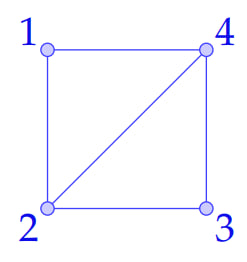
\includegraphics[width=0.7\textwidth]{slides/pic_1.jpg}
        \end{column}
    \end{columns}
\end{frame}
\addtocounter{framenumber}{-1}
%-------------------------------------------------------------
\begin{frame}{2-WL Refinement Algorithm}
    \begin{columns}
        \begin{column}{0.7\textwidth}
        \begin{align*}
            A_2 = \begin{bmatrix}
                a&b&c&b\\
                d&e&d&f\\
                c&b&a&b\\
                d&f&d&e
            \end{bmatrix}
        \end{align*}
        \end{column}

        \begin{column}{0.3\textwidth}
            \centering
            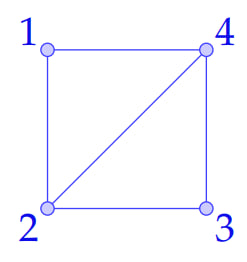
\includegraphics[width=0.7\textwidth]{slides/pic_1.jpg}
        \end{column}
    \end{columns}
    
    \vspace{1em}
    \[
    \scalebox{0.8}{
    $
        A_2^2 = \begin{bmatrix}
            a^2+2bd+c^2 & ab+be+bf+cb&ac+2bd+ca & ab+be+bf+cb\\
            da+dc+ed+fd&2db+e^2+f^2&da+dc+ed+fd&2db+ef+fe\\
            ac+2bc+ca&ab+be+bf+cb&a^2+2bd+c^2&ab+be+bf+cb\\
            da+dc+ed+fd & 2db+ef+fe & da+dc+ed+fd & 2db+e^2+f^2
        \end{bmatrix}
    $
    }
    \]

    % \vspace{1em}
    % \begin{align*}
    %     A_2 = \begin{bmatrix}
    %         a&b&c&b\\
    %         d&e&d&f\\
    %         c&b&a&b\\
    %         d&f&d&e
    %     \end{bmatrix}
    % \end{align*}
\end{frame}
\addtocounter{framenumber}{-1}
%-------------------------------------------------------------
\begin{frame}{2-WL Refinement Algorithm}
    \begin{columns}
        \begin{column}{0.7\textwidth}
        \begin{align*}
            A_2 = \begin{bmatrix}
                a&b&c&b\\
                d&e&d&f\\
                c&b&a&b\\
                d&f&d&e
            \end{bmatrix}
        \end{align*}
        \end{column}

        \begin{column}{0.3\textwidth}
            \centering
            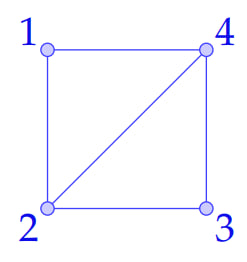
\includegraphics[width=0.7\textwidth]{slides/pic_1.jpg}
        \end{column}
    \end{columns}
    
    \vspace{1em}
    \[
    \scalebox{0.8}{
    $
        A_2^2 = \begin{bmatrix}
            a^2+2bd+c^2 & ab+be+bf+cb&ac+2bd+ca & ab+be+bf+cb\\
            da+dc+ed+fd&2db+e^2+f^2&da+dc+ed+fd&2db+ef+fe\\
            ac+2bc+ca&ab+be+bf+cb&a^2+2bd+c^2&ab+be+bf+cb\\
            da+dc+ed+fd & 2db+ef+fe & da+dc+ed+fd & 2db+e^2+f^2
        \end{bmatrix}
    $
    }
    \]

    \vspace{1em}
    \begin{align*}
        A_3 = \begin{bmatrix}
            a&b&c&b\\
            d&e&d&f\\
            c&b&a&b\\
            d&f&d&e
        \end{bmatrix}
    \end{align*}
\end{frame}
\addtocounter{framenumber}{-1}
%-------------------------------------------------------------
\begin{frame}{2-WL Refinement Algorithm}
    \begin{columns}
        \begin{column}{0.7\textwidth}
        \begin{align*}
            A_2 = \begin{bmatrix}
                a&b&c&b\\
                d&e&d&f\\
                c&b&a&b\\
                d&f&d&e
            \end{bmatrix}
        \end{align*}
        \end{column}

        \begin{column}{0.3\textwidth}
            \centering
            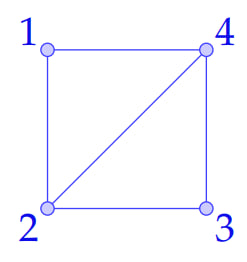
\includegraphics[width=0.7\textwidth]{slides/pic_1.jpg}
        \end{column}
    \end{columns}
    
    \vspace{1em}
    \[
    \scalebox{0.8}{
    $
        A_2^2 = \begin{bmatrix}
            a^2+2bd+c^2 & ab+be+bf+cb&ac+2bd+ca & ab+be+bf+cb\\
            da+dc+ed+fd&2db+e^2+f^2&da+dc+ed+fd&2db+ef+fe\\
            ac+2bc+ca&ab+be+bf+cb&a^2+2bd+c^2&ab+be+bf+cb\\
            da+dc+ed+fd & 2db+ef+fe & da+dc+ed+fd & 2db+e^2+f^2
        \end{bmatrix}
    $
    }
    \]

    \vspace{1em}
    \begin{align*}
        A_3 = \begin{bmatrix}
            a&b&c&b\\
            d&e&d&f\\
            c&b&a&b\\
            d&f&d&e
        \end{bmatrix}=A_2
    \end{align*}
\end{frame}
\addtocounter{framenumber}{-1}
%-------------------------------------------------------------
\begin{frame}{2-WL Refinement Algorithm}
    \begin{columns}
        \begin{column}{0.7\textwidth}
        \begin{align*}
            \mathcal{W}(\Gamma) = \begin{bmatrix}
                a&b&c&b\\
                d&e&d&f\\
                c&b&a&b\\
                d&f&d&e
            \end{bmatrix}
        \end{align*}
        \end{column}

        \begin{column}{0.3\textwidth}
            \centering
            $\Gamma$
            
            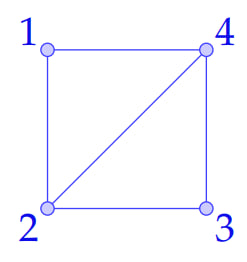
\includegraphics[width=0.7\textwidth]{slides/pic_1.jpg}
        \end{column}
    \end{columns}
    
    \vspace{1em}
    \centering
    \[
    \scalebox{0.7}{
    $
        \begin{array}{cccccc}
        a & b & c & d & e & f \\
        \begin{bmatrix}
        1&0&0&0\\
        0&0&0&0\\
        0&0&1&0\\
        0&0&0&0
        \end{bmatrix}
        &
        \begin{bmatrix}
        0&1&0&1\\
        0&0&0&0\\
        0&1&0&1\\
        0&0&0&0
        \end{bmatrix}
        &
        \begin{bmatrix}
        0&0&1&0\\
        0&0&0&0\\
        1&0&0&0\\
        0&0&0&0
        \end{bmatrix}
        &
        \begin{bmatrix}
        0&0&0&0\\
        1&0&1&0\\
        0&0&0&0\\
        1&0&1&0
        \end{bmatrix}
        &
        \begin{bmatrix}
        0&0&0&0\\
        0&1&0&0\\
        0&0&0&0\\
        0&0&0&1
        \end{bmatrix}
        &
        \begin{bmatrix}
        0&0&0&0\\
        0&0&0&1\\
        0&0&0&0\\
        0&1&0&0
        \end{bmatrix}
        \end{array}
    $
    }
    \]

    \vspace{1em}
    \centering
    We say "$\Gamma$ has \textbf{coherent rank} 6".
\end{frame}
\addtocounter{framenumber}{-1}

%---------------------------------------------------------
% \begin{frame}{Why Study Coherent Closures?}
%   \textbf{Applications:}
%   \begin{itemize}
%     \item \textbf{Chemistry:} Molecular symmetry detection;
%     \item \textbf{Network Science:} Role-based structure in graphs;
%     \item \textbf{Quantum Computing:} Qubit interaction graphs via association schemes.
%   \end{itemize}
% \end{frame}

%---------------------------------------------------------
\begin{frame}{Choice of Base Graph}
We want graphs with a known coherent rank, such as 

\textbf{strongly regular graphs}.

\vspace{1em}
\textbf{Strongly regular graphs} are a class of simple graphs $G=(V,E)$, with the following properties.
\begin{itemize}
    \item Total vertices: $|V| = v$;
    \item Each vertex has degree $k$;
    \item For every pair of adjacent vertices, they share $\lambda$ common adjacent vertices;
    \item For every pair of non-adjacent vertices, they share $\mu$ common adjacent vertices;
    \item Known coherent rank of 3, with the coherent closure having basis matrices $\langle I, A, J-I-A\rangle$.
\end{itemize}

From here, we refer to such strongly regular graphs with the parameters above as $\operatorname{SRG}(v,k,\lambda,\mu)$.
\end{frame}
%---------------------------------------------------------
\begin{frame}{Choice of Base Graph}
\textbf{Base Graph:} The Rook graph \( R(n) \), induced from OA(2,n).

\vspace{1em}
\textbf{Properties}
        \begin{itemize}
            \item $|V|=n^2, |E|=2(n-1)$;
            \item Strongly regular with parameters $\operatorname{SRG}(n^2,2(n-1),n-2,2)$;
            \item Interpreted as the possible moves of a Rook on a $n\times n$ chessboard.
        \end{itemize}
\end{frame}

%---------------------------------------------------------
\begin{frame}{Graph Operations Studied}
We investigate how the coherent closure \( \mathcal{W} \) containing the adjacency matrix of a graph $G=(V,E)$ evolves under two structural graph modifications:

\vspace{1em}
\textbf{1. Vertex Deletion},
% \begin{itemize}
%     \item Choose a vertex $v\in V$ and remove that vertex from the graph, and all its incident edges.
%     \item The resulting graph is $G'=(V',E')$, where $V'=V\setminus\{v\}$.
% \end{itemize}

\vspace{1em}
\textbf{2. Seidel Switching}.
% \begin{itemize}
%   \item Select subset \( S \subseteq V \); flip adjacency between \( S \) and \( V \setminus S \)
%   \item Edges within \( S \) and \( V \setminus S \) remain unchanged
% \end{itemize}
\end{frame}

%---------------------------------------------------------
\begin{frame}{Graph Operation: Vertex Deletion}
\textbf{Vertex Deletion:}
\begin{itemize}
  \item Choose a vertex \( v \in V \),
  \item Remove \( v \) and all edges incident to it,
  \item The resulting graph is \( G' = (V \setminus \{v\}, E') \).
\end{itemize}

\vspace{1em}
\textbf{Adjacency Matrix Perspective:}
\[
A(G) =
\begin{bmatrix}
0 & \vec{a}^T\\
\vec{a}&A_{11}
\end{bmatrix}
\quad
\Rightarrow
\quad
A(G') = A_{11}
\]
where $A_{11}$ is the adjacency matrix of the resulting graph, and $\vec{a}$ represents the adjacency between $v$ and $V\setminus\{v\}$.
\end{frame}

%---------------------------------------------------------
\begin{frame}{Graph Operation: Seidel Switching}
\textbf{Seidel Switching:}
\begin{itemize}
  \item Choose a subset \( S \subseteq V \),
  \item Flip adjacency between \( S \) and \( V \setminus S \),
  \item Edges within \( S \) and within \( V \setminus S \) are unchanged.
\end{itemize}

\vspace{1em}
\textbf{Adjacency Matrix Perspective:}
\[
A(G) =
\begin{bmatrix}
A(G^S) & C \\
C^T & A(G^{V\setminus S})
\end{bmatrix}
\quad
\Rightarrow
\quad
A(G') =
\begin{bmatrix}
A(G^S) & J-C \\
J-C^T & A(G^{V\setminus S})
\end{bmatrix}
\]
where $A(G^S)$ represents edges in the set $S$, $A(G^{V\setminus S})$ represents edges in the set $V\setminus S$, and $C$ represents the adjacency between vertices in sets $S$ and $V\setminus S$.
\end{frame}

%----------------------------------------------------------
\begin{frame}
    \begin{theorem}[Wielandt's Principle]
        Let $\mathcal{A}$ be a coherent algebra and let $A\in\mathcal{A}$. For $b\in\mathbb{C}$, define the matrix $B$ such that
        \[
        [B]_{xy}=\begin{cases}
            1,\quad \text{if } [A]_{xy}=b;\\
            0,\quad \text{otherwise}.
        \end{cases}
        \]
        then, $B\in\mathcal{A}$.
    \end{theorem}
\end{frame}

%----------------------------------------------------------
\begin{frame}{Process of finding coherent closure}

Showing upper bound:
\begin{enumerate}
    \item Use 2-WL refinement algorithm for small $n$,
    \item Notice pattern and generalise into a set of basis matrices and show they form a coherent algebra, $\mathcal{A}$.
\end{enumerate}

\vspace{1em}
Showing Lower bound:
\begin{enumerate}
    \item Use the Wielandt's Principle to show that a certain number of basis matrices need to exist in the coherent closure,
    \item Show that the minimum number of basis matrices is equal to $|\mathcal{A}|$, and thus $\mathcal{W}=\mathcal{A}$.
\end{enumerate}
\end{frame}

%----------------------------------------------------------
\begin{frame}{Summary of Coherent Rank and Types}
\centering
\begin{tabular}{|c|c|c|}
\hline
\textbf{Graph Operation} & \textbf{Coherent Rank} & \textbf{Type} \\
\hline
Vertex Deletion & 10 & $\begin{bmatrix} 3 & 2 \\ 2 & 3 \end{bmatrix}$ \\
\hline
Switching on 1 Vertex & 15 & 
$\begin{bmatrix}
1 & 1 & 1 \\
1 & 3 & 2 \\
1 & 2 & 3
\end{bmatrix}$ \\
\hline
Switching on 1 $n$-clique & 10 & 
$\begin{bmatrix}
2 & 2 \\
2 & 4
\end{bmatrix}$ \\
\hline
Switching on $1<k<\frac{n}{2}$ $n$-cliques & 12 & 
$\begin{bmatrix}
4 & 2 \\
2 & 4
\end{bmatrix}$ \\
\hline
Switching on $\frac{n}{2}$ $n$-cliques & 6 & $[6]$ \\
\hline
\end{tabular}

\[
\begin{aligned}
    A(R(n)) = 
    \left[
        \begin{array}{cccc}
        J_{n} - I & I_n & \cdots & I_n \\
        I_n & J_n - I & \cdots & I_n \\
        \vdots & \vdots & \ddots & \vdots \\
        I_n & I_n & \cdots & J_n - I
        \end{array}
    \right]
\end{aligned}
\]
\end{frame}



%----------------------------------------------------------
% put key findings all into 1 slide below
%----------------------------------------------------------
% \begin{frame}{Vertex Deletion on R(n), $\Gamma_1$}
% \vspace{1em}
% \begin{columns}
%     \begin{column}{0.6\textwidth}
%         \textbf{Key Findings:}
%         \begin{itemize}
%         \item There are 2 induced sub-graphs:
%             \begin{itemize}
%                 \item $A_1$ is the adjacency matrix of 2 disjoint $K_{n-1}$.
%                 \item $A_2$ is the adjacency matrix of $R(n-1)$.
%             \end{itemize}
%         \item Both sub-graphs are strongly regular
%         \end{itemize}
%     \end{column}

%     \begin{column}{0.4\textwidth}
%         \begin{align*}
%             A(\Gamma_1) = \begin{bmatrix}
%                 A_1&C\\C^T&A_2
%             \end{bmatrix}
%         \end{align*}
%     \end{column}
% \end{columns}
% \end{frame}

% \begin{frame}{$\mathcal{W}(\Gamma_1)$}
% We have the following 10 basis matrices:
% \begin{align*}
% W_1 &= 
% \begin{bmatrix}
% I & O \\
% O & O
% \end{bmatrix},
% & \quad
% W_2 &= 
% \begin{bmatrix}
% O & O \\
% O & I
% \end{bmatrix}, \\
% W_3 &= 
% \begin{bmatrix}
% A_1 & O \\
% O & O
% \end{bmatrix},
% & \quad
% W_4 &= 
% \begin{bmatrix}
% O & O \\
% O& A_2
% \end{bmatrix}, \\
% W_5 &= 
% \begin{bmatrix}
% J-I-A_1 & O \\
% O & O
% \end{bmatrix},
% & \quad
% W_6 &= 
% \begin{bmatrix}
% O & O \\
% O & J-I-A_2
% \end{bmatrix},\\
% W_7 &= 
% \begin{bmatrix}
% O & C \\
% O & O
% \end{bmatrix},
% & \quad
% W_8 &= 
% \begin{bmatrix}
% O & O \\
% C^T & O
% \end{bmatrix},\\
% W_9 &= 
% \begin{bmatrix}
% O& J-C \\
% O & O
% \end{bmatrix},
% & \quad
% W_{10} &=
% \begin{bmatrix}
% O& O \\
% J-C^T & O
% \end{bmatrix}.
% \end{align*}

% The coherent rank of $\Gamma_1$ is 10.
% \end{frame}


% %---------------------------------------------------------
% \begin{frame}{Observed Coherent Rank and Structure}
% \textbf{After Vertex Deletion from \( R(4,4) \):}
% \begin{itemize}
%   \item Coherent rank remains \textbf{15}, same as the original graph
%   \item Basis matrices partitioned into 2 substructures:
%   \begin{itemize}
%     \item One diagonal block: \( (n-1) \times (n-1) \) identity and offset blocks
%     \item Other diagonal block: fibre-related structure, zero blocks and projections
%   \end{itemize}
% \end{itemize}

% \vspace{1em}
% \textbf{Interpretation:}
% \begin{itemize}
%   \item Suggests structural resilience in adjacency algebra
%   \item Patterns suggest deeper regularity in OA-derived graphs
% \end{itemize}
% \end{frame}

%---------------------------------------------------------
% \begin{frame}{Seidel Switching on Rook Graphs}

% \vspace{1em}
% \textbf{Key Findings:}
% \begin{itemize}
%   \item Switching a \textbf{single vertex} $\Rightarrow$ coherent rank = \textbf{15}
%   \item Switching \textbf{\( n/2 \) disjoint \( n \)-cliques} $\Rightarrow$ coherent rank = \textbf{6}
%   \item Switching \( k \) disjoint \( n \)-cliques with \( 1 < k < n/2 \) $\Rightarrow$ coherent rank = \textbf{12}
% \end{itemize}
% \end{frame}

%---------------------------------------------------------
\begin{frame}{Interpreting Coherent Rank Patterns}

Other graphs considered:

\vspace{1em}
\begin{columns}
\begin{column}{0.3\textwidth}
\centering
    Block Graph of OA($3,n$)

    \vspace{1em}
    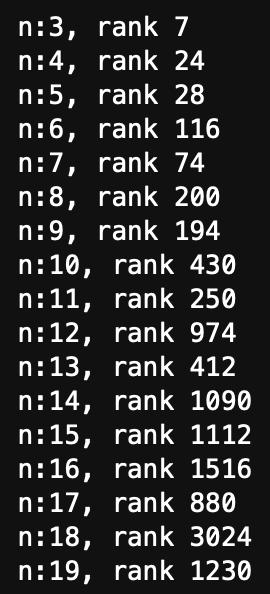
\includegraphics[height=5cm]{slides/OA(3,n).jpg}
\end{column}

\begin{column}{0.3\textwidth}
\centering
    Triangular Graph, $T(n)$
    
    \vspace{1em}
    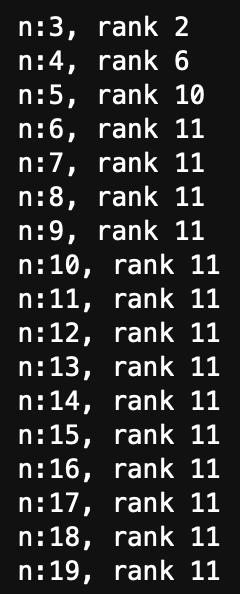
\includegraphics[height=5cm]{slides/T(n).jpg}
\end{column}

\begin{column}{0.3\textwidth}
\centering
    Paley Graph, 
    
    $P(n)$
    
    \vspace{1em}
    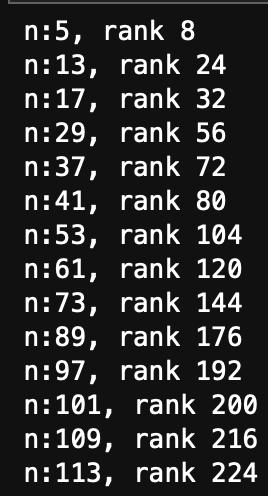
\includegraphics[height=5cm]{slides/Paley.jpg}
\end{column}
\end{columns}

% \textbf{What does coherent rank reflect?}
% \begin{itemize}
%   \item Encodes the number of basis relations in \( \mathcal{W}(G) \)
%   \item Lower rank $\Rightarrow$ more collapsed structure or indistinguishable vertices
%   \item Higher rank $\Rightarrow$ finer structural distinction preserved
% \end{itemize}

% \vspace{1em}
% \textbf{Key Insight:}
% \begin{itemize}
%     \item For $R(n)$, graph operations such as vertex deletion and seidel switching can result in a general coherent closure of the respective modified graphs.
%     \item Even by destroying regularity in a strongly regular graph, we are able to find a stable combinatorial structure for the graphs.
% \end{itemize}
\end{frame}


%---------------------------------------------------------
\begin{frame}{Conclusion and Future Directions}
\textbf{Summary:}
\begin{itemize}
  \item Studied coherent closures of modified rook graphs;
  \item Applied vertex deletion and Seidel switching;
  \item Observed fixed coherent rank and algebraic structure under graph operations.
\end{itemize}

\vspace{1em}
\textbf{Future Work:}
\begin{itemize}
  \item Extend analysis to larger \( k \), higher-order OA$(k,n)$;
  \item Extend analysis to other strongly regular graphs, such as Triangular graphs or Paley graphs.
\end{itemize}

\vspace{1em}
\centering
\textit{Thank you! I welcome your questions.}
\end{frame}




% %---------------------------------------------------------
% \begin{frame}{Q\&A}
%   Thank you! I'm happy to take any questions.
% \end{frame}

\end{document}
